%%%%%%%%%%%%%%%%%%%%%%%%%%%%%%%%%%%%%%%%%
% Short Sectioned Assignment LaTeX Template Version 1.0 (5/5/12)
% This template has been downloaded from: http://www.LaTeXTemplates.com
% Original author:  Frits Wenneker (http://www.howtotex.com)
% License: CC BY-NC-SA 3.0 (http://creativecommons.org/licenses/by-nc-sa/3.0/)
%%%%%%%%%%%%%%%%%%%%%%%%%%%%%%%%%%%%%%%%%

%----------------------------------------------------------------------------------------
%	PACKAGES AND OTHER DOCUMENT CONFIGURATIONS
%----------------------------------------------------------------------------------------

\documentclass[paper=a4, fontsize=11pt]{scrartcl} % A4 paper and 11pt font size

% ---- Entrada y salida de texto -----

\usepackage[T1]{fontenc} % Use 8-bit encoding that has 256 glyphs
\usepackage[utf8]{inputenc}

% ---- Idioma --------

\usepackage[spanish, es-tabla]{babel} % Selecciona el español para palabras introducidas automáticamente, p.ej. "septiembre" en la fecha y especifica que se use la palabra Tabla en vez de Cuadro

% ---- Otros paquetes ----

% Hipervínculos
\usepackage[hidelinks]{hyperref}

\usepackage{amsmath,amsfonts,amsthm} % Math packages
\usepackage{graphics,graphicx, float, url} %para incluir imágenes y colocarlas
% \usepackage{ulem}

\usepackage{fancyhdr} % Custom headers and footers
\pagestyle{fancyplain} % Makes all pages in the document conform to the custom headers and footers
\fancyhead{} % No page header - if you want one, create it in the same way as the footers below
\fancyfoot[L]{} % Empty left footer
\fancyfoot[C]{} % Empty center footer
\fancyfoot[R]{\thepage} % Page numbering for right footer
\renewcommand{\headrulewidth}{0pt} % Remove header underlines
\renewcommand{\footrulewidth}{0pt} % Remove footer underlines
\setlength{\headheight}{13.6pt} % Customize the height of the header

\numberwithin{equation}{section} % Number equations within sections (i.e. 1.1, 1.2, 2.1, 2.2 instead of 1, 2, 3, 4)
\numberwithin{figure}{section} % Number figures within sections (i.e. 1.1, 1.2, 2.1, 2.2 instead of 1, 2, 3, 4)
\numberwithin{table}{section} % Number tables within sections (i.e. 1.1, 1.2, 2.1, 2.2 instead of 1, 2, 3, 4)

\setlength\parindent{0pt} % Removes all indentation from paragraphs - comment this line for an assignment with lots of text

\newcommand{\horrule}[1]{\rule{\linewidth}{#1}} % Create horizontal rule command with 1 argument of height

%% Para incluir archivos en texto plano
\usepackage{listings}

%----------------------------------------------------------------------------------------
%	TÍTULO Y DATOS DEL ALUMNO
%----------------------------------------------------------------------------------------

\title{	
\normalfont \normalsize 
\textsc{{\bf Ingeniería de Servidores (2015-2016)} \\ Doble Grado en Ingeniería Informática y Matemáticas \\ Universidad de Granada} \\ [25pt] % Your university, school and/or department name(s)
\horrule{0.5pt} \\[0.4cm] % Thin top horizontal rule
\huge Memoria Práctica 4 \\ % The assignment title
\horrule{2pt} \\[0.5cm] % Thick bottom horizontal rule
}

\author{Óscar Bermúdez Garrido\\ \href{http://www.github.com/oxcar103}{@oxcar103}} % Nombre y apellidos

\date{\normalsize\today} % Incluye la fecha actual

%----------------------------------------------------------------------------------------
% DOCUMENTO
%----------------------------------------------------------------------------------------

\begin{document}
\maketitle % Muestra el Título
\newpage %inserta un salto de página
\tableofcontents % para generar el índice de contenidos
\listoffigures

\newpage

\begin{enumerate}
	\section{Benchmarks populares}
	\subsection{Phoronix Suite}
		\item Instale la aplicación. ¿Qué comando permite listar los benchmarks disponibles?
		
		\textit{Phoronix Test Suite} es una software multiplataforma de evaluación de rendimiento
		desarrollado por \textit{Phoronix Media}\cite{phoronix_official} y distribuido mediante la 
		licencia de software libre \href{https://www.gnu.org/licenses/gpl.html}{\textbf{GPL}}
		
		Instalaremos la aplicación mediante \textit{sudo apt-get install phoronix-test-suite}). Tras
		esto, consultamos el manual \cite{man_phoronix} y vemos que podemos deplegar una lista completa
		de los posibles benchmarks con el parámetro \textit{list-available-tests}, de entre los que
		escogeremos en el siguiente punto.
		
		\item \textbf{Opcional:} Seleccione, instale y ejecute uno, comente los resultados\footnote{No
		es lo mismo un benchmark que una suite, instale un benchmark}.
		
		Como para Windows escogí un benchmark de memoria, ahora cogeré uno de otra cosa.
		
		De entre la lista disponible, me llamó mucho la atención uno de criptografía, \textit{gcrypt},
		que pone a prueba el procesador.
		
		Para ejecutar un benchmark, hay que escribir \textit{phoronix-test-suite benchmark $<$nombre$>$}.
		
		Tras esto, se descarga los archivos necesario\footnote{Esto se debe a que tenerlos todos
		descargados haría que el paquete fuese increíblemente pesado porque, de los benchmarks que
		muestra el parámetro \textit{list-available-tests}, algunos de dichos tests son juegos para
		probar la tarjeta gráfica, lo que puede suponer fácilmente 0.5 GB por juego\footnote{Nótese
		además que hay otro comando disponible llamado \textit{list-available-suites} que permite ver
		algunos bancos de pruebas, con lo cuál, el peso sería aún mayor.}.}, y empieza la ejecución
		preguntando primero si se quiere guardar en algún lugar específico el resultado.
		
		Durante la ejecución, se realizan varias mediciones y se toma la media junto con la desviación
		típica de los datos para el cuál podemos ver que se han necesitado 8350 microsegundos de medio
		para 6 ejecuciones del benchmark de encriptación con una desviación típica de $7.11\%$:
		
		\begin{figure}[H]
			\centering
			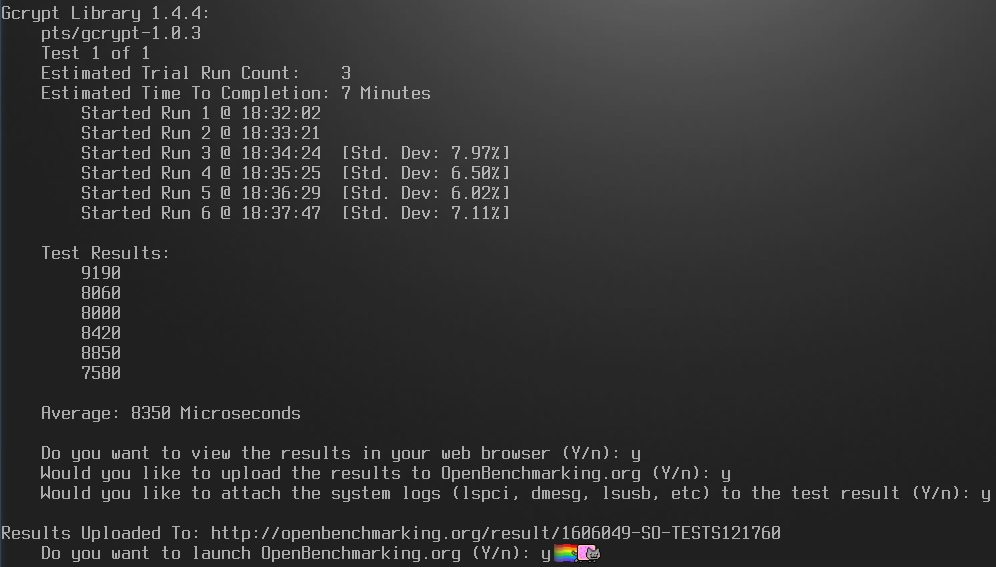
\includegraphics[width=15cm]{Ejercicio_2.jpg}
			\caption{Resultados del benchmark escogido.}
			\label{fig:phoronix}
		\end{figure}
		
		Al finalizar, se sugiere mostrar los resultados en el navegador(y si quieres subirlos a la
		página oficial).
		
	\subsection{Benchmarks y Test de Estrés para Webs}
	\subsubsection{Apache Benchmarks}
		\item De los parámetros que le podemos pasar al comando, ¿qué significa \textit{-c 5}?
		¿y \textit{-n 100}? Monitorice la ejecución de \textit{ab} contra alguna máquina (cualquiera),
		¿cuántos procesos o hebras crea \textit{ab} en el cliente?
		
		\textit{ab} es una herramienta de benchmarking diseñada para testear el servidor Apache HTTP
		por la \textit{Fundación Apache}\cite{apache_official} y distribuida mediante la licencia de
		software libre \href{https://www.apache.org/licenses/LICENSE-2.0}{\textbf{Apache License}}.
		
		Para conocer el significado de los parámetros, simplemente miramos el manual \cite{man_ab} y
		vemos que \textit{-c} cambia el número de peticiones simultáneas que se pueden lanzar, 5 en
		nuestro caso, y que \textit{-n} nos permite configurar cuántas peticiones totales queremos
		realizar, 100 para nuestro ejemplo\footnote{Investigando el manual por mi cuenta para otro
		trabajo\cite{TWG}, también descubrí algunos parámetros que pueden resultar útiles como pueden
		ser \textit{-b} para cambia el tamaño de la ventana de mensajes TCP, \textit{-t} para marcar
		un tiempo límite para el benchmark en lugar de un número de mensajes límite y \textit{-e} que
		permite escribir un fichero en formato \textit{csv}.}.
		
		Monitorizando con \textit{htop}\cite{man_htop}, añadiendo la columna \textit{NLWP} que es la
		que nos muestra el número de hebras que utiliza cada proceso y filtrando por nombre del comando
		podemos ver el número de hebras que necesita, que dependerá del número de peticiones simultáneas
		se le permitan ejecutar.
		
		\item Ejecute \textit{ab} contra las 3 máquinas virtuales (desde el SO anfitrión a las máquinas
		virtuales de la red local en Ubuntu, CentOS y WS) una a una (arrancadas por separado) y muestre
		y comente las estadísticas. ¿Cuál es la que proporciona mejores resultados? Fíjese en el número
		de bytes transferidos, ¿es igual para cada máquina?
		
		El resultado de la ejecución de \textit{ab} sería:
		
		\begin{itemize}
			\item \textbf{Ubuntu:}
			\lstinputlisting{./Ubuntu.txt}
			
			\item \textbf{Windows Server:}
			\lstinputlisting{./WS.txt}
			
			\item \textbf{CentOS}
			\lstinputlisting{./CentOS.txt}
		\end{itemize}
		
		Como podemos observar, los resultados de las máquinas son muy bajos, por lo que les estaría
		afectando en gran parte el ruido. Si suponemos que no se ha captado apensa ruido, podemos
		concluir que el más rápido sería en nuestro caso \textit{Ubuntu}, seguido de \textit{CentOS}
		y \textit{Windows Server}, respectivamente. Este hecho quizás sea posible ya que la máquina
		anfitrión es una variante de Ubuntu y, por tanto, tenga una mayor compatibilidad. Además,
		podemos ver que el número de bytes transferidos difiere siendo el menor el de \textit{Windows
		Server}, seguido de \textit{Ubuntu} y \textit{CentOS}.
		
	\subsubsection{Gatling}
		\item \textbf{Opcional:} ¿Qué es Scala? Instale Gatling y pruebe los escenarios por defecto.
		
		Scala\cite{Scala} es un lenguaje de programación diseñado para ser conciso, orientado a objetos
		al igual que Java y con gran soporte para programación funcional.
		
	\subsubsection{Jmeter}
		\item \textbf{Opcional:} Lea el artículo y elabore un breve resumen.
		En este artículo\cite{flood_article}, Tim Koopmans compara \textit{JMeter} y \textit{Gatling},
		según su propia palabra, las dos herramientas de evaluación de rendimiento de código abierto
		disponibles más populares.
		
		Antes de nada, pasa a describirnos el escenario sobre el que se realizarán las pruebas\footnote{
		Básicamente, se puede resumir en Ubuntu como sistema operativo, 10000 usuarios, 30000 peticiones
		por minutos un nodo de \textit{flood.io}\footnotemark que 
		equivale 15 GB de RAM, un procesador de 64 bit con 4 núcleos.}\footnotetext[6]{Básicamente, un
		poco de autopublicidad.}.
		
		Tras el experimento, se deduce que ha poca diferencia entre ambas herramientas pues se obtuvieron
		unos resultados muy similares con ligeras diferencias:
		\begin{itemize}
			\item \textit{Jmeter} utiliza más recursos, tanto de procesador como memoria.
			\item \textit{Gatling} tiene más problemas de concurrencia.
		\end{itemize}
		
		Especialmente, me parece curiosa la sección \textit{TL;DR}\footnote{Acrónimo de \textit{Too
		Long; Don't Read}} que básicamente ya nos hace el resumen del artículo.
		
		\item Instale y siga el tutorial en \url{http://jmeter.apache.org/usermanual/build-web-test-plan.html}
		realizando capturas de pantalla y comentándolas. En vez de usar la web de \textit{jmeter},
		haga el experimento usando alguna de sus máquinas virtuales (Puede hacer una página sencilla,
		usar las páginas de \textit{phpmyadmin}, instalar un \textit{CMS}, \dots).
		
		Para instalar \textit{JMeter}, nos bastará con hacer uso del gestor de paquetes por defecto, en
		mi caso sería \textit{apt-get}, para instalar el paquete de nombre \textit{jmeter}.
		
		Tras instalarlo y, aunque no es mi caso, configurarlo inicialmente para que se adapte al uso que
		posteriormente se le dará, procedemos a ejecutarlo\footnote{Sería conveniente previamente echar
		un vistazo a su manual \cite{man_jmeter} aunque por mi parte no encontré nada especialmente de
		interés aunque para una integración a un trabajo más serio que éste, pues esto no es más que un
		experimento de juguete para tomar contacto con la herramienta, es bastante probable que dichas
		funcionalidades sean de interés.}.
		
		Siguiendo el tutorial proporcionado, vemos que el primer paso sería definir el conjunto de
		usuarios que utilizaremos para esta prueba. Para esto, haremos click derecho en la batería de
		pruebas definidas por el usuario como podemos ver en la imagen:
		
		\begin{figure}[H]
			\centering
			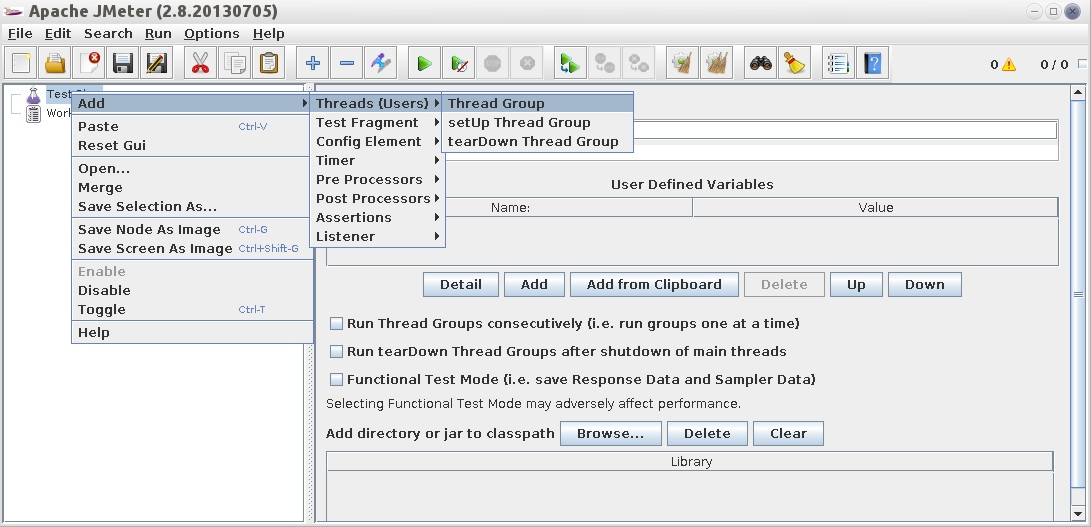
\includegraphics[width=15cm]{Ejercicio_7a.jpg}
			\caption{Abrimos el menú de creación de usuarios.}
			\label{fig:user_menu}
		\end{figure}
		
		Dentro de este menú, configuramos a placer algunas de las características del grupo de usuarios
		que queremos emular, así como el número de ellos que simularemos, el intervalo de tiempo que
		estableceremos entre el inicio de un usuario y el siguiente, el número de iteraciones que
		ejecutaremos,... Por defecto, el tutorial nos indica que modifiquemos el nombre, el número de
		usuarios y el número de iteraciones tal y como se nos muestra:
		
		\begin{figure}[H]
			\centering
			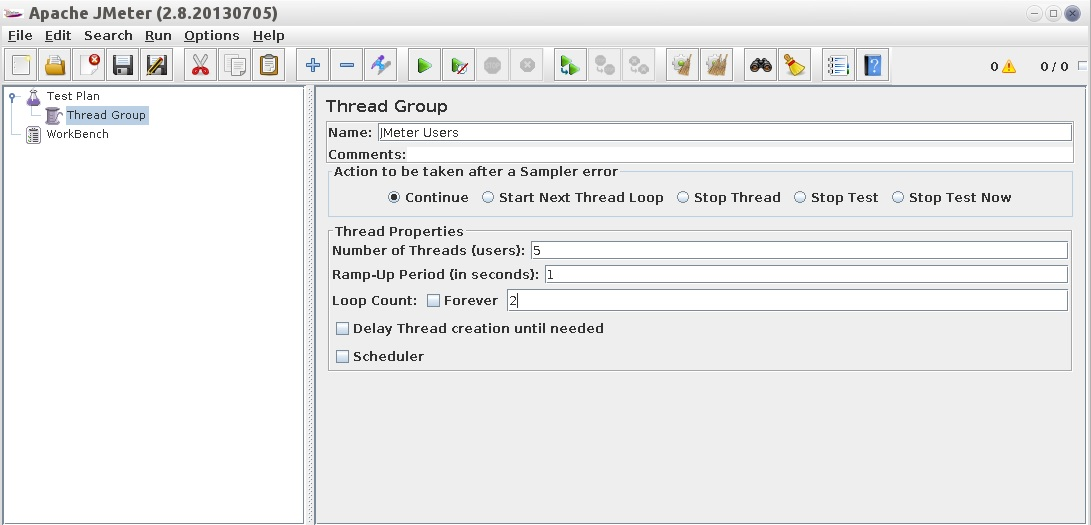
\includegraphics[width=15cm]{Ejercicio_7b.jpg}
			\caption{Configuración del \textit{Thread Group}.}
			\label{fig:user_config}
		\end{figure}
		
		Dentro de este grupo, crearemos unos parámetros por defecto para configuraciones HTTP, para
		ello, previamente haremos click derecho en el grupo para añadirlo como podemos ver en la
		siguiente imagen:
		
		\begin{figure}[H]
			\centering
			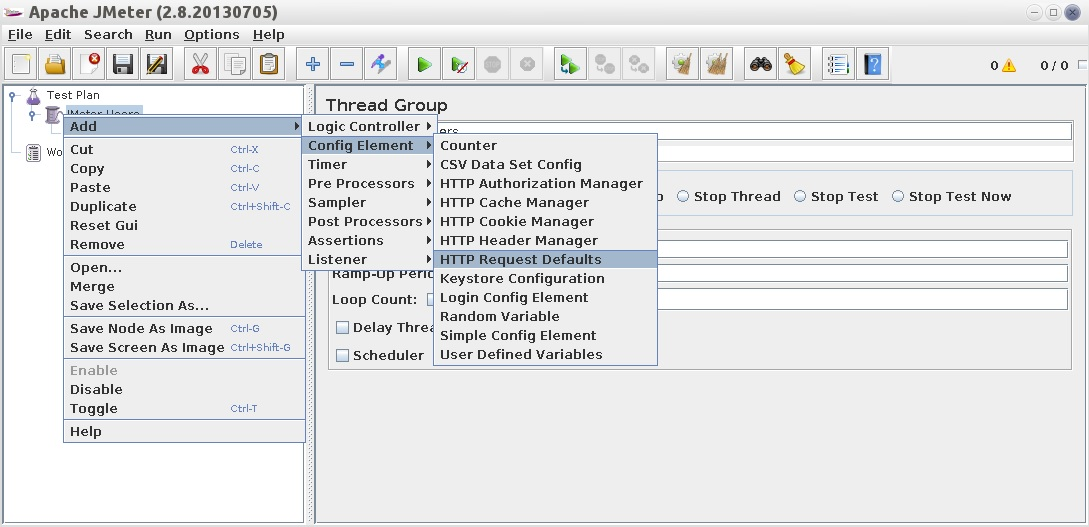
\includegraphics[width=15cm]{Ejercicio_7c.jpg}
			\caption{Abrimos el menú de configuración de peticiones HTTP.}
			\label{fig:http_menu}
		\end{figure}
		
		\begin{figure}[H]
			\centering
			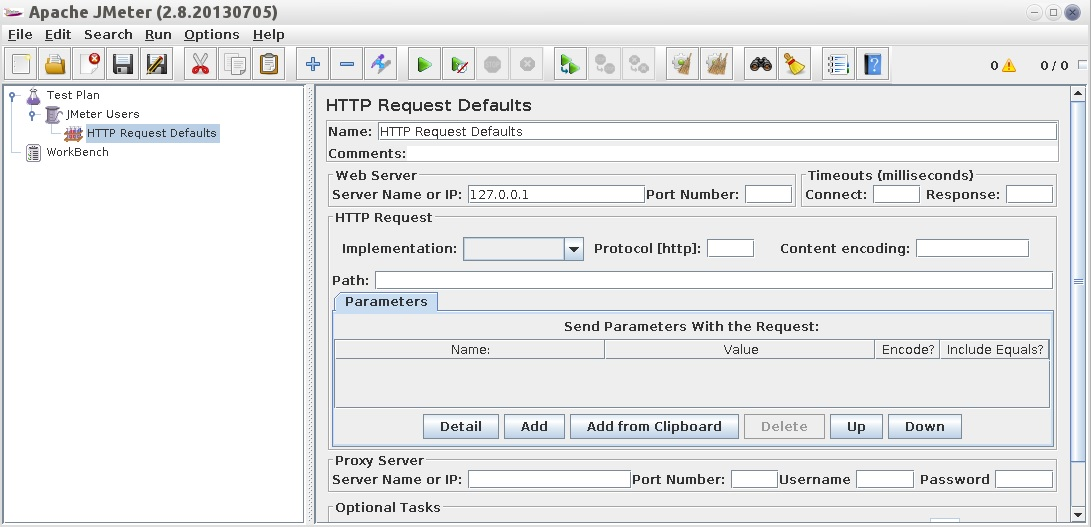
\includegraphics[width=15cm]{Ejercicio_7d.jpg}
			\caption{Resultados del benchmark escogido.}
			\label{fig:phoroix}
		\end{figure}
		
		\begin{figure}[H]
			\centering
			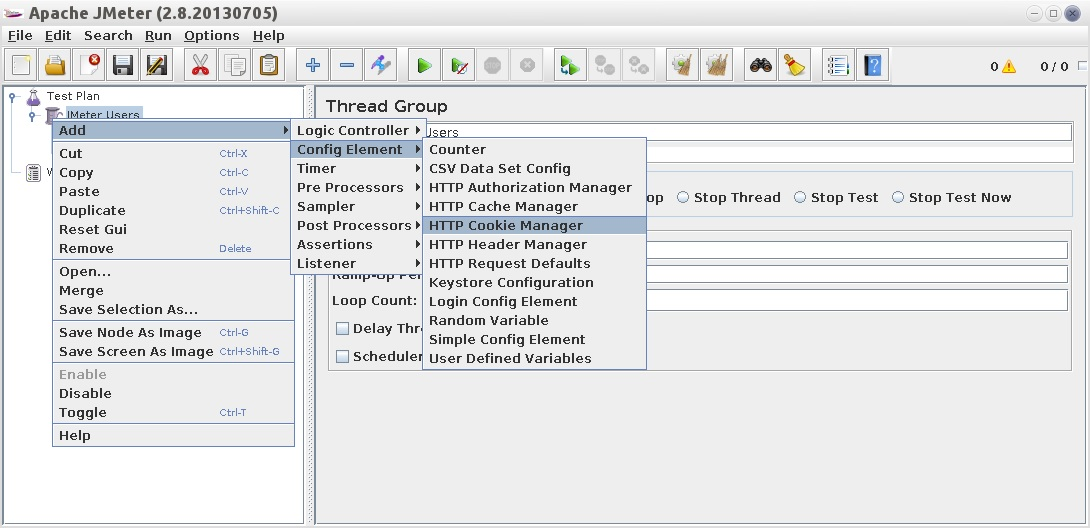
\includegraphics[width=15cm]{Ejercicio_7e.jpg}
			\caption{Resultados del benchmark escogido.}
			\label{fig:phorox}
		\end{figure}
		
		\begin{figure}[H]
			\centering
			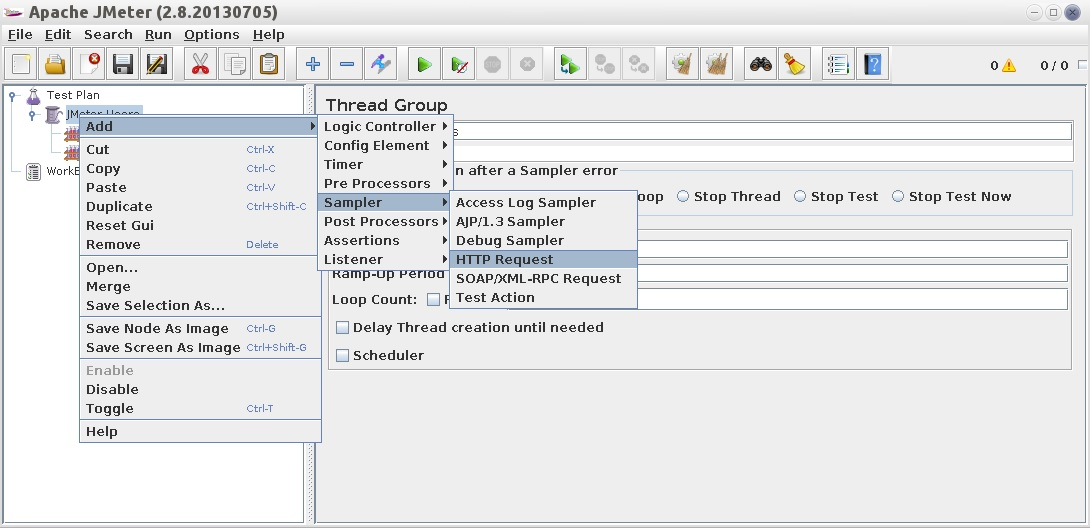
\includegraphics[width=15cm]{Ejercicio_7f.jpg}
			\caption{Resultados del benchmark escogido.}
			\label{fig:phoroi}
		\end{figure}
		
		\begin{figure}[H]
			\centering
			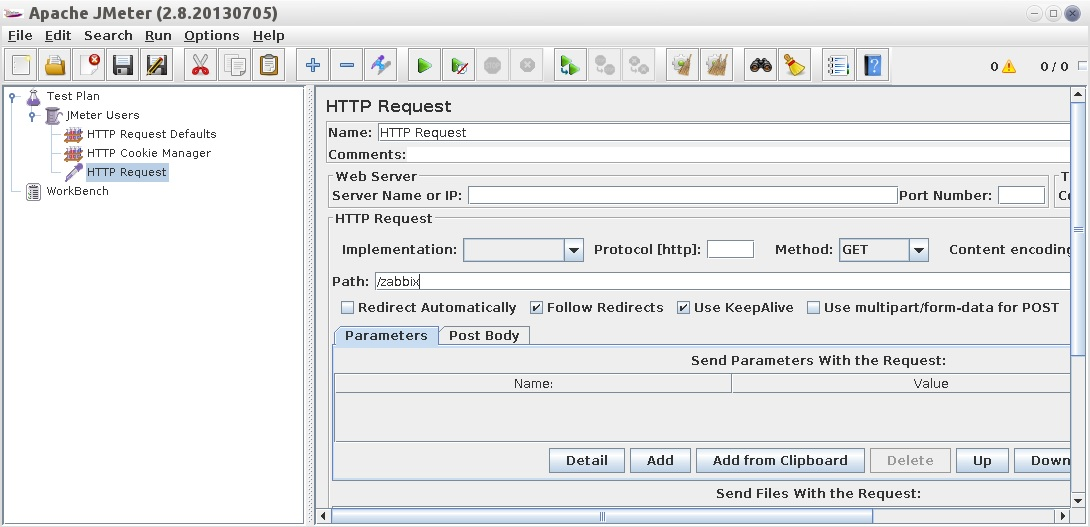
\includegraphics[width=15cm]{Ejercicio_7g.jpg}
			\caption{Resultados del benchmark escogido.}
			\label{fig:phoro}
		\end{figure}
		
		\begin{figure}[H]
			\centering
			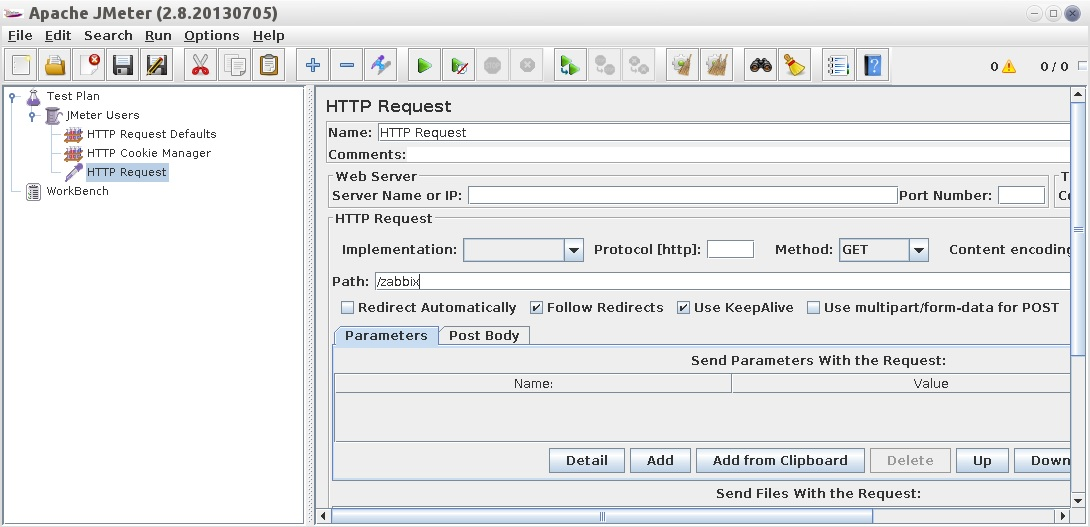
\includegraphics[width=15cm]{Ejercicio_7h.jpg}
			\caption{Resultados del benchmark escogido.}
			\label{fig:phor}
		\end{figure}
		
		\begin{figure}[H]
			\centering
			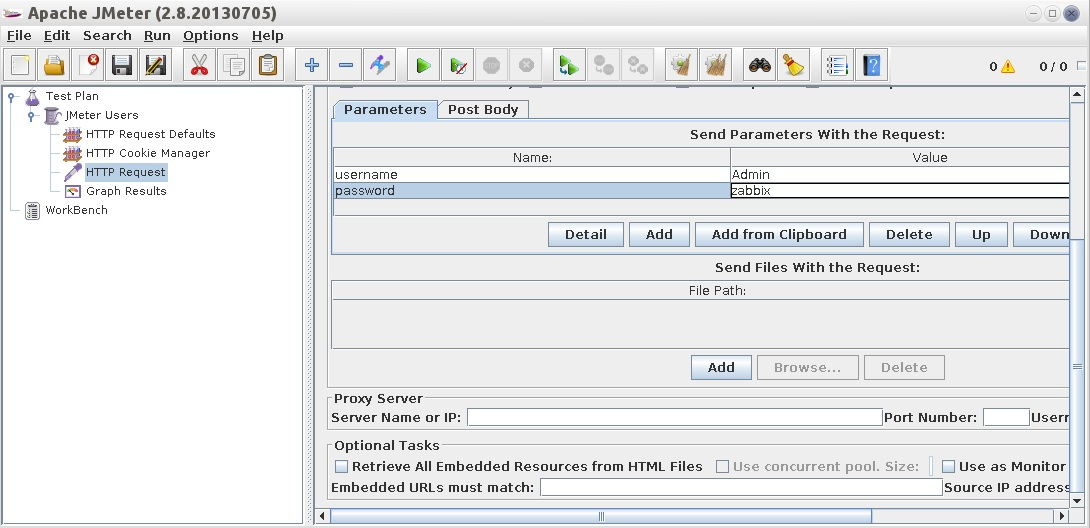
\includegraphics[width=15cm]{Ejercicio_7i.jpg}
			\caption{Resultados del benchmark escogido.}
			\label{fig:phori}
		\end{figure}
		
		\begin{figure}[H]
			\centering
			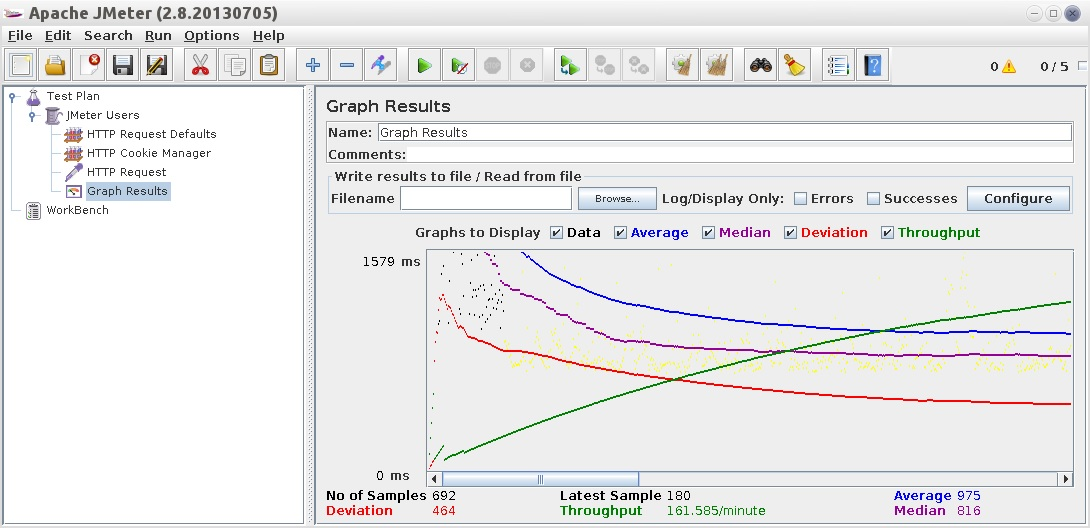
\includegraphics[width=15cm]{Ejercicio_7j.jpg}
			\caption{Resultados del benchmark escogido.}
			\label{fig:phorn}
		\end{figure}
		
		
	\subsection{Benchmarks para Windows}
	\subsubsection{Sisoftware Sandra}
	\subsubsection{AIDA64 (Antiguo Everest)}
		\item \textbf{Opcional:} Seleccione un benchmark entre \textit{SisoftSandra} y \textit{Aida}.
		Ejecútelo y muestre capturas de pantalla comentando los resultados.
		
		Tras instalar Aida, vamos al apartado de Benchmark y seleccionamos el que queremos dentro de
		los disponibles. Yo he elegido uno de copia en memoria porque me ha parecido bastante completo
		al tener que leer y escribir.
		
		Los resultados aparecen con una comparativa de otras máquinas(datos que vienen por defecto en
		el programa) bastante heterogéneas entre sí.
		
		Nuestra máquina, aparece con un color distinto al de las demás para poder distinguirla sin
		necesidad de conocer todas las características de la misma a la perfección:
		
		\begin{figure}[H]
			\centering
			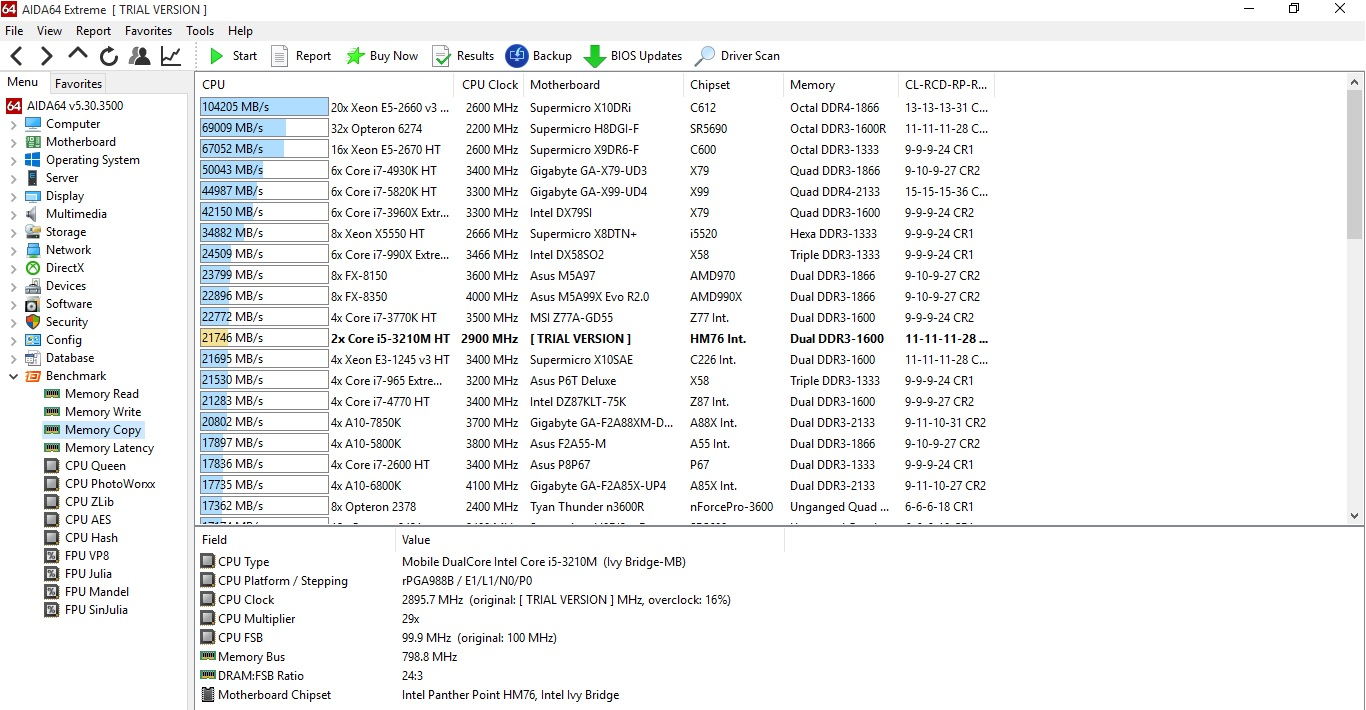
\includegraphics[width=15cm]{Ejercicio_8.jpg}
			\caption{Resultados del benchmark escogido.}
			\label{fig:Aida}
		\end{figure}
		
	\subsection{Más Benchmarks\dots}
		\item Programe un benchmark usando el lenguaje que desee. El benchmark debe incluir:
		\begin{enumerate}
			\item Objetivo del benchmark.
			\item Métricas (unidades, variables, puntuaciones, \dots).
			\item Instrucciones para su uso.
			\item Ejemplo de uso analizando los resultados.
		\end{enumerate}
		Tenga en cuenta que puede comparar varios gestores de BD, lenguajes de programación web (tiempos
		de ejecución, gestión de memoria, \dots), duración de la batería, servidor DNS, \dots,
		Alternativamente, puede descargar alguno de algún repositorio en GitHub y modificarlo según sus
		necesidades.
		
\end{enumerate}

\newpage
\section{Referencias}
\begin{thebibliography}{10}
\expandafter\ifx\csname url\endcsname\relax
  \def\url#1{\texttt{#1}}\fi
\expandafter\ifx\csname urlprefix\endcsname\relax\def\urlprefix{URL }\fi
\expandafter\ifx\csname href\endcsname\relax
  \def\href#1#2{#2} \def\path#1{#1}\fi

\bibitem{man_yum}
Ubuntu manuals\\
yum(8) - Linux man page\\
\url{http://manpages.ubuntu.com/manpages/xenial/en/man8/yum.8.html}

\bibitem{man_yum.conf}
Ubuntu manuals\\
yum.conf(5) - Linux man page\\
  \url{http://manpages.ubuntu.com/manpages/xenial/en/man5/yum.conf.5.html}

\bibitem{CentOS_web}
CentOS.org\\
10. Using yum with a Proxy Server\\
  \url{https://www.centos.org/docs/5/html/yum/sn-yum-proxy-server.html}

\bibitem{foro_Fedora}
Fedoraforum.org\\
A fedora linux support community\\
  \url{http://forums.fedoraforum.org/showthread.php?t=742}

\bibitem{man_yum-config-manager}
Ubuntu manuals\\
yum-config-manager(1) - Linux man page\\
  \url{http://manpages.ubuntu.com/manpages/xenial/en/man1/yum-config-manager.1.html}

\bibitem{man_apt-cache}
Ubuntu manuals\\
apt-cache(8) - Linux man page\\
  \url{http://manpages.ubuntu.com/manpages/xenial/en/man8/apt-cache.8.html}

\bibitem{man_apt-get}
Ubuntu manuals\\
apt-get(8) - Linux man page\\
  \url{http://manpages.ubuntu.com/manpages/xenial/en/man8/apt-get.8.html}

\bibitem{man_apt.conf}
Ubuntu manuals\\
apt.conf(5) - Linux man page\\
  \url{http://manpages.ubuntu.com/manpages/wily/en/man5/apt.conf.5.html}

\bibitem{man_add-apt-repository}
Ubuntu manuals\\
add-apt-repository\\
  \url{http://manpages.ubuntu.com/manpages/natty/man1/add-apt-repository.1.html}

\bibitem{man_apt}
Ubuntu manuals\\
apt(8) - Linux man page\\
  \url{http://manpages.ubuntu.com/manpages/xenial/en/man8/apt.8.html}

\bibitem{oS_packman}
The openSUSE wiki\\
Package Management\\
  \url{https://en.opensuse.org/Package_management}

\bibitem{oS_YaST}
The openSUSE wiki\\
YaST Software Management\\
  \url{https://en.opensuse.org/Portal:YaST}

\bibitem{oS_zypper}
The openSUSE wiki\\
Zypper\\
  \url{https://en.opensuse.org/Portal:Zypper}

\bibitem{oS_YaST_GitHub}
GitHub - How people build software\\
YaST\\
  \url{https://github.com/yast}

\bibitem{oS_zypper_GitHub}
GitHub - How people build software\\
Zypper - Según su propia descripción: "World's most powerful command line package manager"\\
  \url{https://github.com/openSUSE/zypper}

\bibitem{Telnet}
Telnet. Wikipedia, the free encyclopedia.\\
  \url{https://en.wikipedia.org/wiki/Telnet}

\bibitem{SSH}
Secure Shell. Wikipedia, the free encyclopedia.\\
  \url{https://en.wikipedia.org/wiki/Secure_Shell}

\bibitem{man_SSH}
Ubuntu manuals\\
ssh(1) - Linux man page\\
  \url{http://manpages.ubuntu.com/manpages/xenial/en/man1/ssh.1.html}

\bibitem{SSH_StackOverFlow}
StackOverFlow. \\
How to SSH to a VirtualBox guest externally through a host? \\
  \url{http://stackoverflow.com/questions/5906441/how-to-ssh-to-a-virtualbox-guest-externally-through-a-host}

\bibitem{man_ssh-keygen}
Ubuntu manuals\\
ssh-keygen(1) - Linux man page\\
  \url{http://manpages.ubuntu.com/manpages/xenial/en/man1/ssh-keygen.1.html}

\bibitem{man_ssh-copy-id}
Ubuntu manuals\\
ssh-copy-id(1) - Linux man page\\
  \url{http://manpages.ubuntu.com/manpages/xenial/en/man1/ssh-copy-id.1.html}

\bibitem{man_apropos}
Ubuntu manuals\\
apropos(1) - Linux man page\\
  \url{http://manpages.ubuntu.com/manpages/xenial/en/man1/apropos.1.html}

\bibitem{man_service}
Ubuntu manuals\\
service(8) - Linux man page\\
  \url{http://manpages.ubuntu.com/manpages/xenial/en/man8/service.8.html}

\bibitem{man_systemctl}
Ubuntu manuals\\
systemctl(1) - Linux man page\\
  \url{http://manpages.ubuntu.com/manpages/xenial/en/man1/systemctl.1.html}

\bibitem{man_fail2ban}
Ubuntu manuals\\
fail2ban(1) - Linux man page\\
  \url{http://manpages.ubuntu.com/manpages/xenial/en/man1/fail2ban.1.html}

\bibitem{man_jail.conf}
Ubuntu manuals\\
jail.conf(5) - Linux man page\\
  \url{http://manpages.ubuntu.com/manpages/xenial/en/man1/jail.conf.10.html}

\bibitem{man_sshd_config}
Ubuntu manuals\\
sshd\_config(5) - Linux man page\\
  \url{http://manpages.ubuntu.com/manpages/xenial/en/man5/sshd_config.5.html}

\bibitem{man_nano}
Ubuntu manuals\\
nano(1) - Linux man page\\
  \url{http://manpages.ubuntu.com/manpages/xenial/en/man1/nano.1.html}

\bibitem{TWG}
GitHub - How people build software\\
Análisis comparativo de Tomcat, WildFly y GlassFish\\
  \url{https://github.com/oxcar103/Trabajo-ISE}

\bibitem{TC_official}
\textbf{Apache Tomcat}\\
  \url{http://tomcat.apache.org/}

\bibitem{WF_official}
\textbf{JBossDeveloper}\\
  \url{http://wildfly.org/}\\
  \url{http://jbossas.jboss.org/}\footnote{Antiguo enlace a la página oficial, al parecer, esta página
  ha dejado de estar disponible, luego éste ya no está operativo pero me parece que tiene cierto
  interés histórico.}\\

\bibitem{GF_official}
\textbf{GlassFish}\\
  \url{https://glassfish.java.net/}

\bibitem{GF_install}
\textbf{\textit{Java EE 7 with GlassFish 4 Application Server}}\\
David R. Heffelfinger\\
Ed. Packt Publishing (March 2014)\\
Sec. "1. Getting Started with GlassFish"\\
  \url{http://proquest.safaribooksonline.com/book/programming/java/9781782176886}

\bibitem{TC_install}
\textbf{\textit{Apache Tomcat 7 Essentials}}\\
Tanuj Khare\\
Ed. Packt Publishing (March 2012)\\
Sec. "1. Installation of Tomcat7"\\
  \url{http://proquest.safaribooksonline.com/book/operating-systems-and-server-administration/apache/9781849516624}

\bibitem{TC_download}
\textbf{Apache Tomcat}\\
  \url{http://tomcat.apache.org/download-70.cgi}

\bibitem{TC_StackOverFlow}
\textbf{Stack Overflow}
  \url{http://stackoverflow.com/questions/4756039/how-to-change-the-port-of-tomcat-from-8080-to-80}

\bibitem{WF_install}
\textbf{\textit{WildFly: New Features}}\\
Filippe Costa Spolti\\
Ed. Packt Publishing (May 2014)\\
Sec. "1. Starting with WildFly"\\
  \url{http://proquest.safaribooksonline.com/9781783285891?uicode=goliat} 

\bibitem{WF_download}
\textbf{JBossDeveloper}\\
  \url{http://wildfly.org/downloads/}

\bibitem{WF_solution}
\textbf{Dmitriy Sukharev. IT Blog}\\
  \url{http://sukharevd.net/wildfly-8-installation.html}
  \url{https://gist.github.com/sukharevd/6087988}

\bibitem{man_diff}
Ubuntu manuals\\
diff(1) - Linux man page\\
  \url{http://manpages.ubuntu.com/manpages/xenial/en/man1/diff.1posix.html}

\bibitem{man_patch}
Ubuntu manuals\\
patch(1) - Linux man page\\
  \url{http://manpages.ubuntu.com/manpages/xenial/en/man1/patch.1.html}

\bibitem{webmin}
Webmin.com\\
Using the Webmin APT repository\\
  \url{http://webmin.com/deb.html}

\bibitem{man_php}
Ubuntu manuals\\
php(1) - Linux man page\\
  \url{http://manpages.ubuntu.com/manpages/precise/en/man1/php.1.html}

\bibitem{ispconfig}
ispconfig.org\\
Online demo\\
  \url{http://www.ispconfig.org/ispconfig/online-demo/}

\bibitem{man_find}
Ubuntu manuals\\
find(1) - Linux man page\\
  \url{http://manpages.ubuntu.com/manpages/xenial/en/man1/find.1.html}

\bibitem{man_grep}
Ubuntu manuals\\
grep(1) - Linux man page\\
  \url{http://manpages.ubuntu.com/manpages/xenial/en/man1/grep.1posix.html}

\bibitem{man_sed}
Ubuntu manuals\\
sed(1) - Linux man page\\
  \url{http://manpages.ubuntu.com/manpages/xenial/en/man1/sed.1posix.html}

\bibitem{man_awk}
Ubuntu manuals\\
awk(1) - Linux man page\\
  \url{http://manpages.ubuntu.com/manpages/xenial/en/man1/awk.1plan9.html}

\end{thebibliography}


\end{document}